\documentclass[t,ignorenonframetext]{beamer}
%\usepackage{beamerthemeJuanLesPins}%
%\usepackage{beamercolorthemecougar} 
%\usepackage{beamerinnerthemecircles} 
\mode<presentation>
{
  \usetheme{Darmstadt}
  \usecolortheme{rose}
  \usefonttheme{default}
}

%\usefonttheme{structuresmallcapsserif}
\usepackage{enumerate,graphicx,verbatim,url}
\usepackage{fancyvrb}
\usepackage{graphicx}
\usepackage{algorithmic}


\newcommand\Red[1]{\textcolor{red}{#1}}

\usepackage{tikz}
\usetikzlibrary{arrows,decorations.pathmorphing,fit,positioning}

% The line below is what I talked about that makes all
% items in a list into overlays
%\beamerdefaultoverlayspecification{<+->}

\newcommand{\tc}[1]{$\backslash$\texttt{#1}}
\newcommand{\specialcell}[2][c]{%
  \begin{tabular}[#1]{@{}c@{}}#2\end{tabular}}
  
\title{Lyrics-based Musical Genre Analysis using LDA}
\author{David van Erkelens, Elise Koster \& Sharon Gieske}
\begin{document}
\frame{
\maketitle
}
\frame{
\tableofcontents
}

\section[Introduction]{Introduction}

\subsection{Motivation}
\begin{frame}
\frametitle{Motivation}
\begin{itemize}
	\item Online music services $\rightarrow$ personalized suggestions based on genre, collective intelligence
	\item Most music classification tasks based on audio signals $\rightarrow$ more storage, more noise-sensitive
	\item Earlier research did not use Topic Models for classification
	\item Applications: automatic genre assignment, finding songs with similar lyrical themes, generating lyrics, modeling correlation between genres based on topic distributions
\end{itemize}
\end{frame}

\subsection{Research Question}
\begin{frame}
\frametitle{Research Question}
Can LDA be used to provide meaningful information about the lyrical themes in different musical genres?


\end{frame}

\section[Approach]{Approach}
\subsection{Methods}
\begin{frame}

\frametitle{Methods}
\begin{itemize}
	\item Latent Dirichlet Allocation: each document has a distribution over topics, and each topic has a distribution over words (see next slide for graphical model)
	\item Gibbs sampling: sample $(topic,word)$ given $p(topic|word)$ and $p(word|topic)$
	\item Every genre now has a distribution over topics, and every topic has a distribution over words
	\item Train SVM on array of topic-probabilities per document (and its genre)
	\item Generate `song' of length $n$ for genre $g$: select topic $k \sim \theta_g$ then select word $w \sim \varphi_k$, repeat $n$ times
\end{itemize}

\end{frame}

\begin{frame}
\frametitle{Plate Diagram}
\begin{figure}[htp]
  \centering
  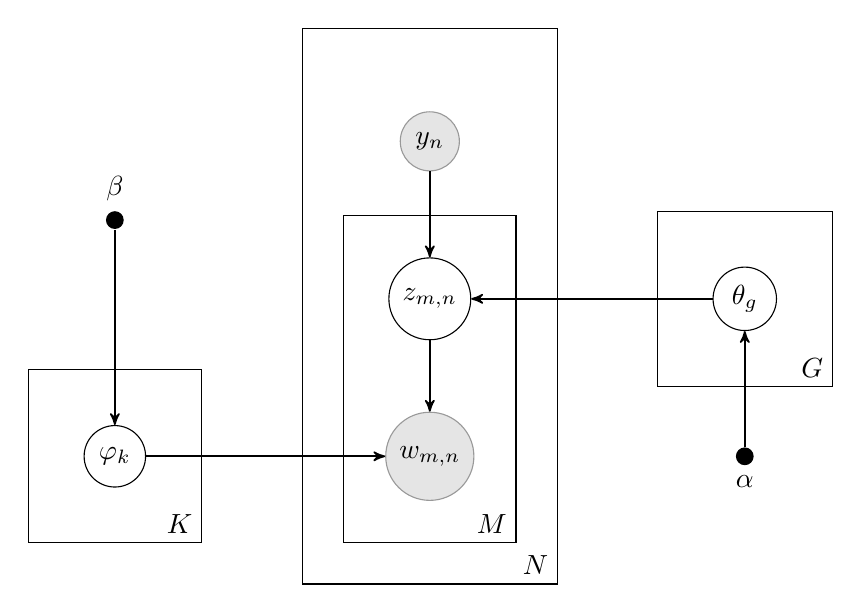
\begin{tikzpicture}
    [
      observed/.style={minimum size=15pt,circle,draw=gray!80,fill=gray!20},
      unobserved/.style={minimum size=15pt,circle,draw},
      hyper/.style={minimum size=1pt,circle,fill=black},
      post/.style={->,>=stealth',semithick},
    ]

    \node (w-j) [observed] at (0,0) {$w_{m,n}$};
    
    \node (z-j) [unobserved] at (0,2) {$z_{m,n}$};

    \node (y) [observed] at (0,4) {$y_n$};
    
    \node (z-prior) [unobserved] at (4,2) {$\theta_g$};
    
    \node (w-prior) [unobserved] at (-4,0) {$\varphi_k$};
    
    \node (z-hyper) [label=below:$\alpha$] at (4,0) {};
    
    \filldraw [black] (4,0) circle (3pt);
    
    \node (w-hyper) [label=above:$\beta$] at (-4,3) {};
    
    \filldraw [black] (-4,3) circle (3pt);
    
    \path
    (z-j) edge [post] (w-j)
    
    (z-hyper) edge [post] (z-prior)
    (z-prior) edge [post] (z-j)
    (y) edge [post] (z-j)


    (w-hyper) edge [post] (w-prior)
    
    (w-prior) edge [post] (w-j)
    ;

    \node [draw,fit=(w-j) (y), inner sep=30pt] (plate-context) {};
    \node [above left] at (plate-context.south east) {$N$};
    \node [draw, fit=(w-prior), inner sep=20pt] (plate-prior) {};
    \node [above left] at (plate-prior.south east) {$K$};
    \node [draw,fit=(w-j) (z-j), inner sep=15pt] (plate-token) {};
    \node [above left] at (plate-token.south east) {$M$};
    \node [draw, fit=(z-prior), inner sep=20pt] (plate-z-prior) {};
    \node [above left] at (plate-z-prior.south east) {$G$};

  \end{tikzpicture}
  \caption{Graphical model}
  \label{fig:graphical-model}
\end{figure}


\end{frame}


\section[Results]{Results}
\subsection{Preliminary Results}
\begin{frame}
\begin{itemize}
	\item Baseline classifier: SVM trained on word counts $\sim 47 \%$ correctly classified.
	\item \begin{tabular}{|c|c|}
		\hline
		Correctly classified &  3154\\
		\hline
		Incorrectly classified & 3574\\
		\hline
		\end{tabular}
	\item Top topic (defined by its top 20 words) for some genres (after 20 iterations):
	\item \begin{tabular} {|c|l|}
	\hline
	Religious & \specialcell{'lord', 'god', 'praise', 'jesus', 'holy', 'every', 'verse', \\ 'chorus', 'yes', 'glory', 'grace', 'power', 'know', \\'worthy', 'great', 'worship', \\'hallelujah', 'let', 'things', 'spirit'}\\
	\hline
	Holiday & \specialcell{'la', 'star', 'two', 'wish', 'like', 'bring', 'see', 'even', \\'good', 'never', 'new', 'get', 'something', 'moving',\\ 'let', 'sound', 'keep', 'christmas', 'come', 'little'} \\
	\hline 
	Rap & \specialcell{'nigga', 'bh', 'yo', 'got', 'st', 'niz', 'lil', 'get', 'fuck', \\'like', 'shit', 'fuckin', 'hoes', 'homie', 'niggas', \\ 'bang', 'ay', 'fresh', 'friends', 'first'}\\
	\hline
	\end{tabular}
\end{itemize}

\end{frame}

\begin{frame}
\frametitle{Plans for rest of project}
\begin{itemize}
	\item Test classification on topic distributions
	\item Build generator
\end{itemize}
\end{frame}

\begin{frame}
\frametitle{Challenges and lessons}
\begin{itemize}
	\item Because we had a non-standard topic, we had to crawl our own dataset and clean and process it.
	\item If you re-compute all word counts every time you go over one word in one document, you're gonna have a (long) bad time. (one iteration of Gibbs sampling took more than 3 days..)
	\item Sometimes you think you've improved something, but in reality you just broke it (results went from sensible $\rightarrow$ meaningless, turns out we just printed the wrong things)
	\item LDA is quite a cool algorithm, if you implement it correctly
	\item `Love' is quite a common word in many musical genres. So are the words `chorus', and `verse', but that may have to do with our data pre-processing.
\end{itemize}
\end{frame}

\section{Conclusion}
\subsection{Conclusion}
\begin{frame}
\frametitle{Conclusions}~\\~\\
\begin{itemize}
\setlength{\itemsep}{10pt}\setlength{\itemsep}{5pt}
\item LDA with Gibbs sampling assigns sensical topics to documents
\item Algorithms take quite some time

\end{itemize}
\end{frame}

\section[Questions]{Questions}
\begin{frame}
~ \\~ \\~ \\ ~ \\~ \\
\begin{center}\Huge Questions? \end{center} 
\end{frame}


\end{document}